\section{Resilienz- und Fehlertoleranzstrategien}

Resilienz ist definiert als die Fähigkeit, Teilausfälle zu bewältigen und die Ausführung ohne Absturz fortzusetzen.

Redundanz bezeichnet in technischen Systemen die bewusste Vervielfältigung kritischer Komponenten oder Funktionen,
um die Zuverlässigkeit und Verfügbarkeit des Gesamtsystems zu erhöhen.
Durch diese Mehrfachauslegung kann das System trotz des Ausfalls einzelner Elemente weiterhin ordnungsgemäß
funktionieren.
Dieses Prinzip findet insbesondere in sicherheitskritischen Bereichen Anwendung, um die Ausfallsicherheit
zu gewährleisten.

\begin{figure}[t]
    \centering
    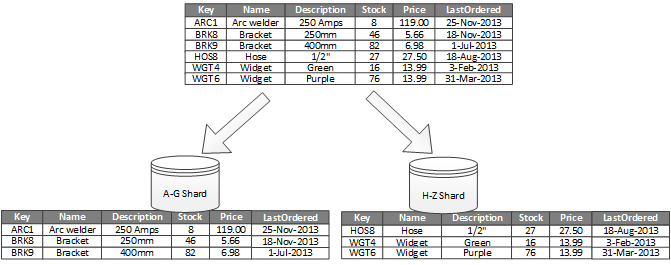
\includegraphics[width=\linewidth]{images/1}
    \caption{XXX}
    \label{fig:1}
\end{figure}

\begin{itemize}
    \item Software-Redundanz: Hierbei werden mehrere Instanzen einer Software parallel betrieben oder unterschiedliche Softwareversionen eingesetzt, um im Fehlerfall auf eine funktionierende Version zurückgreifen zu können. Ein Beispiel ist das N-Version Programming, bei dem mehrere unterschiedliche Implementierungen desselben Algorithmus parallel laufen, um Fehler durch Vergleich der Ergebnisse zu erkennen und zu beheben.
    \item Zeitliche Redundanz: Diese Form der Redundanz beinhaltet die Wiederholung von Prozessen oder Operationen zu verschiedenen Zeitpunkten, um Fehler zu erkennen und zu korrigieren. Durch wiederholte Ausführung kann überprüft werden, ob konsistente Ergebnisse erzielt werden, was insbesondere in Echtzeitsystemen zur Fehlererkennung genutzt wird.
    \item Informationsredundanz (Datenredundanz): Dabei werden zusätzliche Daten gespeichert, die zur Fehlererkennung und -korrektur dienen. Ein Beispiel ist die Speicherung von Paritätsbits in Speichersystemen, die es ermöglichen, fehlerhafte Daten zu identifizieren und zu rekonstruieren.
    \item Hardware-Redundanz: Hier werden physische Komponenten mehrfach vorhanden, um die Ausfallsicherheit zu erhöhen. Dies kann auf verschiedenen Ebenen erfolgen:
    \begin{itemize}
        \item Low-Level-Redundanz: Einsatz redundanter Bauteile innerhalb eines Geräts, wie z.B. mehrfach vorhandene Netzteile oder Lüfter in Servern.
        \item High-Level-Redundanz: Einsatz kompletter zusätzlicher Systeme oder Geräte, wie z.B. parallele Server oder Speichersysteme, die bei Ausfall des Hauptsystems übernehmen können.
    \end{itemize}
\end{itemize}

Durch den gezielten Einsatz dieser Redundanzformen kann die Fehlertoleranz und Verfügbarkeit von Systemen
signifikant gesteigert werden.

%Literature:
%https://www.embedded-software-engineering.de/design-patterns-fuer-hohe-verfuegbarkeit-a-625422/?p=2

Partitionierung ist der Prozess des Aufteilens von Daten oder Workloads in kleinere, unabhängige Segmente,
die separat gespeichert und verarbeitet werden können.
Dies verbessert die Skalierbarkeit, Leistung und Verwaltung von Datenbanken.
Durch die Aufteilung können Daten effizienter verarbeitet und Zugriffe optimiert werden.

\begin{figure}[t]
    \centering
    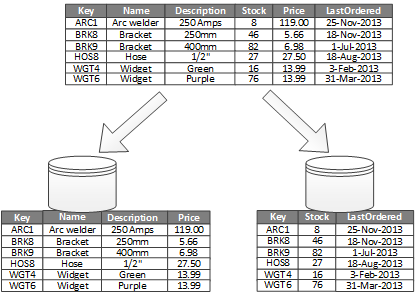
\includegraphics[width=\linewidth]{images/2}
    \caption{XXX}
    \label{fig:2}
\end{figure}

\begin{itemize}
    \item Horizontale Partitionierung (Sharding): Bei dieser Methode werden Datensätze basierend auf bestimmten Kriterien in separate, aber identisch strukturierte Datenbanken oder Tabellen aufgeteilt. Jede Partition, auch “Shard” genannt, enthält eine Teilmenge der Daten, beispielsweise alle Kunden aus einer bestimmten Region. Dies ermöglicht eine nahezu unbegrenzte horizontale Skalierung, da jeder Shard unabhängig verwaltet und auf separaten Servern gehostet werden kann.
    \item Vertikale Partitionierung: Hierbei werden die Spalten einer Tabelle in verschiedene Gruppen aufgeteilt und in separaten Tabellen gespeichert. Häufig genutzte Spalten können in einer Partition zusammengefasst werden, während selten benötigte Daten in einer anderen gespeichert werden. Dies reduziert die Menge der Daten, die bei Abfragen verarbeitet werden müssen, und kann die Leistung verbessern.
    \item Funktionale Partitionierung ist eine Technik, bei der Daten basierend auf der funktionalen Rolle oder dem Zweck, den sie in einem System erfüllen, in separate Partitionen aufgeteilt werden. Wenn ein gebundener Kontext für jeden bestimmten Geschäftsbereich identifiziert werden kann, ist die funktionale Partitionierung eine Möglichkeit zur Verbesserung der Isolation und Datenzugriffsleistung. Darüber hinaus wird die funktionale Partitionierung häufig verwendet, um Lese/Schreibdaten von schreibgeschützten Daten zu trennen.
\end{itemize}

%Literature:
%https://learn.microsoft.com/de-de/azure/architecture/best-practices/data-partitioning

Skalierbarkeit bezeichnet die Fähigkeit eines Systems, einer Anwendung oder eines Netzwerks,
seine Leistung und Kapazität durch Hinzufügen von Ressourcen proportional zur steigenden Nachfrage zu erhöhen.
Ein skalierbares System kann somit effizient auf wachsende Arbeitslasten reagieren, ohne an Leistung einzubüßen.

\begin{figure}[t]
    \centering
    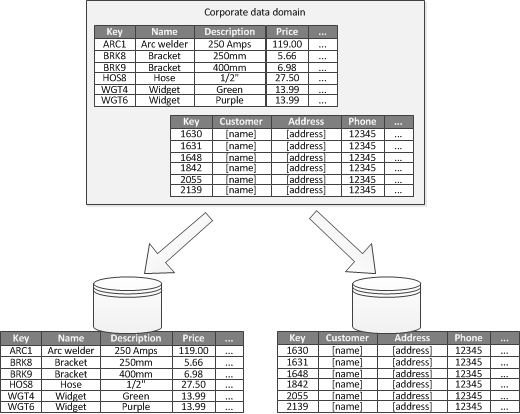
\includegraphics[width=\linewidth]{images/3}
    \caption{XXX}
    \label{fig:3}
\end{figure}

\begin{itemize}
    \item Vertikaler Skalierung (Scale Up): Hierbei werden zusätzliche Ressourcen wie CPU, Arbeitsspeicher oder Speicherplatz zu einem bestehenden Server oder einer bestehenden Instanz hinzugefügt, um die Leistung zu steigern. Ein Beispiel ist das Upgrade eines Datenbankservers mit mehr Arbeitsspeicher, um höhere Anfragen zu bewältigen. In Cloud-Umgebungen kann dies durch den Wechsel zu leistungsfähigeren virtuellen Maschinen erfolgen.
    \item Horizontale Skalierung (Scale Out): Dieser Ansatz fügt dem System zusätzliche Knoten oder Server hinzu, um die Last zu verteilen. Beispielsweise kann ein Webdienst durch Hinzufügen weiterer Server die Anfragen auf mehrere Instanzen verteilen. Dies erfordert oft Lastenausgleichsmechanismen, um den Traffic effizient zu verteilen.
    \item Automatische Skalierung (Autoscaling): Dies bezieht sich auf die dynamische Anpassung der Ressourcen basierend auf der aktuellen Nachfrage. Das System überwacht die Auslastung und fügt bei steigender Nachfrage automatisch Ressourcen hinzu oder reduziert sie bei sinkender Last. Dies gewährleistet Kosteneffizienz und optimale Leistung ohne manuelles Eingreifen.
\end{itemize}

%Literature:
%https://www.ibm.com/think/topics/scale-up-vs-scale-out
%https://azure.microsoft.com/en-us/resources/cloud-computing-dictionary/scaling-out-vs-scaling-up
